
\section{Maidenhead Locator}
\label{section:locator}
\begin{frame}%STARTCONTENT

\frametitle{Problemstellung}
\begin{itemize}
  \item Standort mitteilen, z.B. für Entfernungsmessungen
  \item Es ist nicht immer eine Stadt in der Nähe
  \item GPS-Koordinaten sind zu lang
  \item Oft ist ein ungefährer Standort ausreichend
  \end{itemize}
\end{frame}

\begin{frame}
\frametitle{Maidenhead-Locator}
\begin{itemize}
  \item Erdoberfläche wird in 18.662.400 Kästchen eingeteilt
  \item Ein Kästchen entspricht in Deutschland grob einer Genauigkeit von 5 x \qty{5}{\kilo\metre}
  \item Diese Kästchen werden Subsquare genannt
  \item Übergeordnet sind Squares und Fields
  \end{itemize}

\end{frame}

\begin{frame}
\begin{figure}
    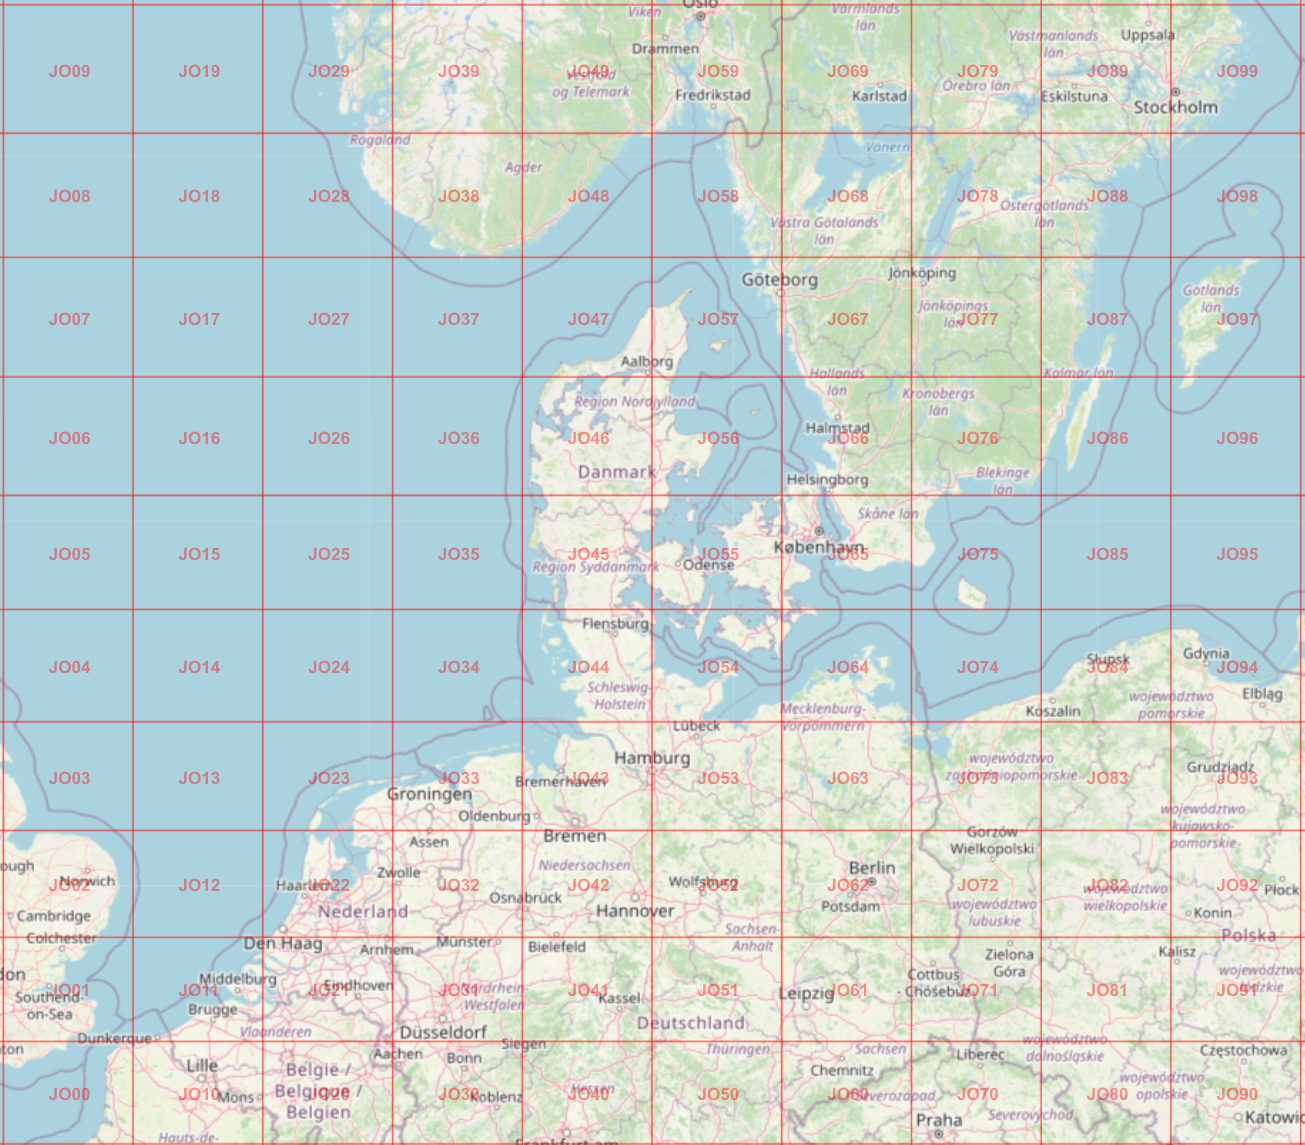
\includegraphics[width=0.85\textwidth]{foto/2}
    \caption{\scriptsize Das Feld JO des Maidenhead-Locator-Systems, Kartendaten © OpenStreetMap-Mitwirkende, SRTM. Kartendarstellung © OpenTopoMap (CC-BY-SA)}
    \label{n_locator_jo}
\end{figure}

\end{frame}

\begin{frame}
\frametitle{Stufen des Maidenhead Locators}
\begin{table}
\begin{DARCtabular}{lllcccc}
     Offizielle Bezeichnung  & Übersetzung  & Alternative Bezeichnung  & & & & Standort DARC   \\
     Field  & Feld  & Größtfeld  & AA  & --  & RR  & JO   \\
     Square  & Quadrat  & Großfeld  & 00  & --  & 99  & 41   \\
     Subsquare  & Unter-Quadrat  & Kleinfeld  & AA  & --  & XX  & RG   \\
\end{DARCtabular}
\caption{Die einzelnen Stufen des Maidenhead-Locators}
\label{n_locator_stufen}
\end{table}
    \pause
    Daraus ergibt sich dann zum Beispiel \emph{JO41RG} für die DARC Geschäftsstelle in Baunatal bei Kassel

\end{frame}

\begin{frame}

\end{frame}

\begin{frame}
\only<1>{
\begin{QQuestion}{BE111}{Was ist der Maidenhead-Locator (auch: QTH-Locator oder Standortkenner)?}{Ein Koordinatensystem, in dem der Standort einer Amateurfunkstelle der zuständigen Behörde mitgeteilt werden muss}
{Eine Positionsangabe durch Verweis auf Felder (fields) und Quadrate (squares), die mit Buchstaben und Ziffern kodiert werden}
{Die Angabe der Standortdaten in Grad, Minuten und Sekunden geographischer Länge und Breite}
{Der geographische Bereich, der sich aus der Zeitzone des Standorts der jeweiligen Amateurfunkstelle ergibt}
\end{QQuestion}

}
\only<2>{
\begin{QQuestion}{BE111}{Was ist der Maidenhead-Locator (auch: QTH-Locator oder Standortkenner)?}{Ein Koordinatensystem, in dem der Standort einer Amateurfunkstelle der zuständigen Behörde mitgeteilt werden muss}
{\textbf{\textcolor{DARCgreen}{Eine Positionsangabe durch Verweis auf Felder (fields) und Quadrate (squares), die mit Buchstaben und Ziffern kodiert werden}}}
{Die Angabe der Standortdaten in Grad, Minuten und Sekunden geographischer Länge und Breite}
{Der geographische Bereich, der sich aus der Zeitzone des Standorts der jeweiligen Amateurfunkstelle ergibt}
\end{QQuestion}

}
\end{frame}%ENDCONTENT
